\documentclass[twoside]{article}
\usepackage{package}
\usepackage[T1]{fontenc}
% Silenciar la advertencia de versalita + negrita inexistente
\WarningFilter{latex}{Some font shapes were not available}
\WarningFilter{latex}{Font shape `T1/lmr/bx/sc'}

% Silenciar la advertencia de caracteres perdidos en el nullfont (para 01_introduccion.tex)
\WarningFilter{latex}{Missing character: There is no}
%Nuevos comandos
\renewcommand{\thefootnote}{\arabic{footnote}}
\raggedbottom



\begin{document}
\begin{center}
    \thispagestyle{empty}
    \large{\textsc{Parámetros en Matlab y Simulink y Funciones Básicas de Control}}\\[0.5cm] 
    \large{Fabrizio Benavidez\footnote[1]{\texttt{fabrizio.benavidez@mi.unc.edu.ar}}}\\[0.5cm]

    \large{\footnotemark[1]\textit{Facultad de Ciencias Exactas, Físicas y Naturales, Ingeniería Aeronáutica}}
    \\[0.5cm]

    \begin{minipage}{0.7\textwidth}
    \hrule
    \vspace{0.2cm}
        \normalsize{\textsc{Resumen}. En el presente trabajo se aborda el modelado dinámico y el análisis de estabilidad de sistemas dinámicos mediante el uso de herramientas computacionales en MATLAB y Simulink. En la primera etapa, se analiza el comportamiento de un modelo de suspensión  de un cuarto de vehículo ante entradas escalón y sinusoidales de diferente frecuencia, evaluando la influencia de los coeficientes de amortiguamiento ($b$) y rigidez ($k$) sobre la respuesta transitoria y la reducción de oscilaciones. En la segunda etapa, se emplea el cálculo simbólico para la obtención de transformadas directas e inversas de Laplace, y se evalúa la estabilidad de sistemas continuos en lazo abierto y lazo cerrado mediante la ubicación de sus polos y ceros en el plano complejo $s$. }\\[0.2cm]
        
        \normalsize{\textit{Palabras claves}: MATLAB, Simulink, Sistemas Dinámicos, Función de Transferencia, Estabilidad, Retroalimentación, Transformada de Laplace. \ }
    \vspace{0.2cm}
    \hrule
    \end{minipage}
    
    \vfil

    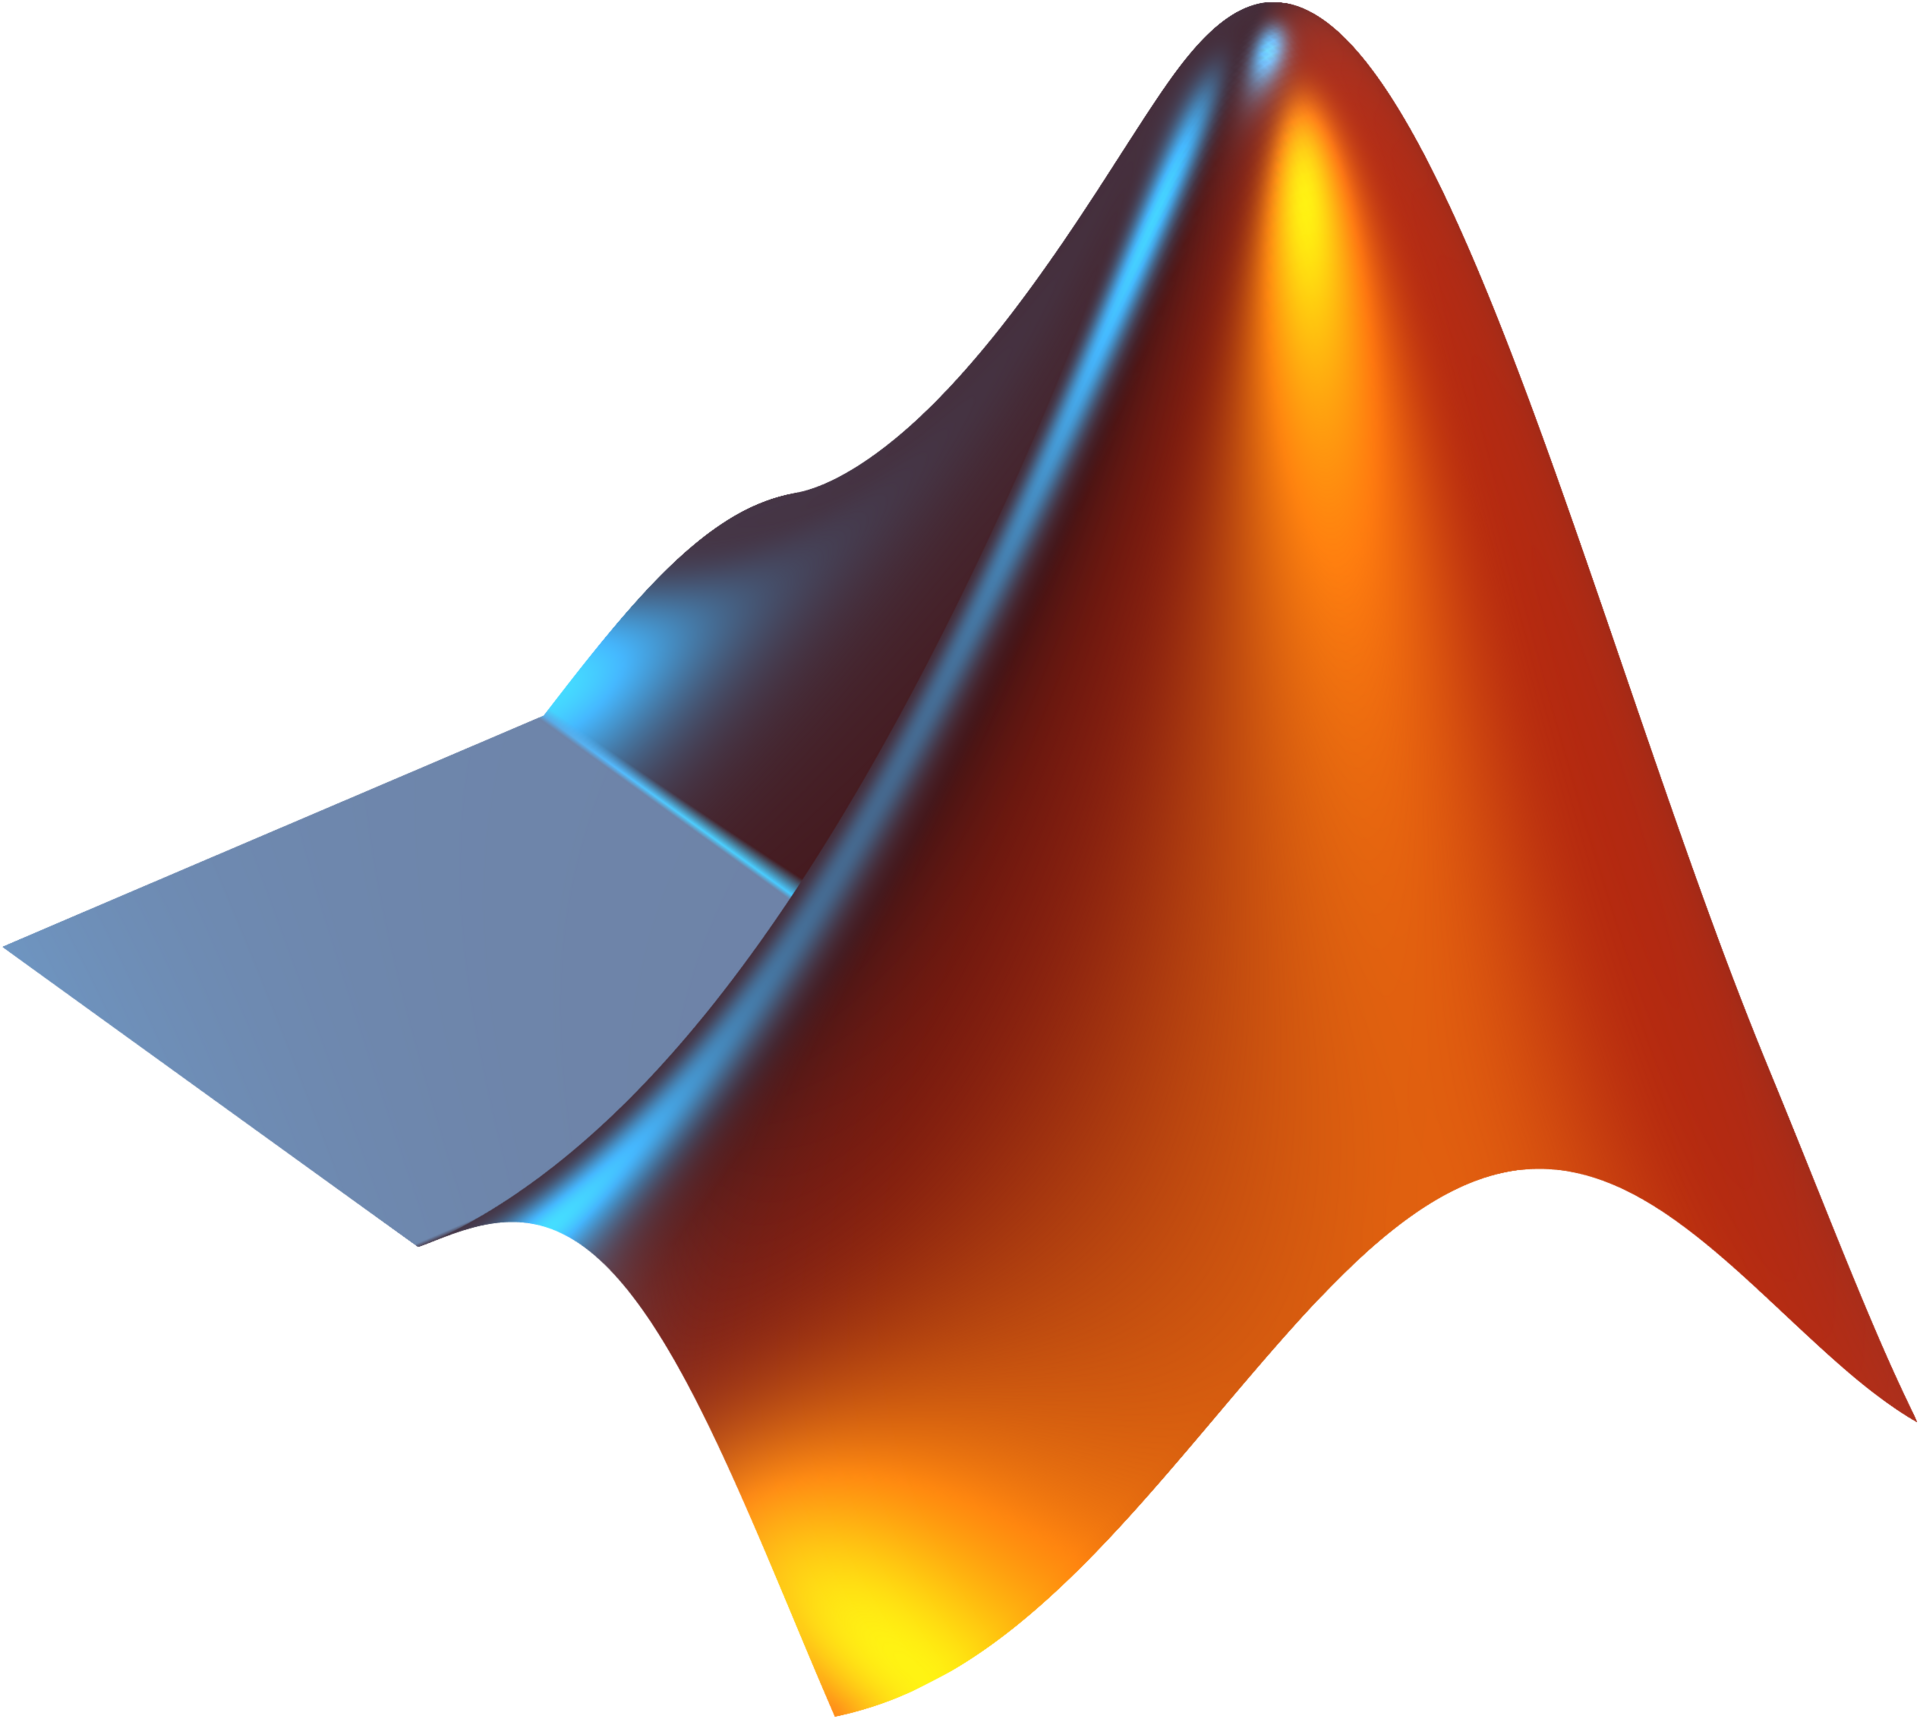
\includegraphics[width = 0.4\textwidth]{imagenes/Matlab_Logo.png}\\[0.5cm]

    \vfil

    \today\\[0.2cm]
    \large{Semana 2}
\end{center}




\newpage

\section{Guía 03}


Consideremos la siguiente figura

\begin{figure}[ht!]
    \centering
    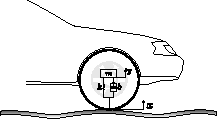
\includegraphics[width = 0.7\textwidth]{imagenes/dibujo_auto.pdf}
    \caption{Esquema de un auto y su modelo del sistema de suspensión}
    \label{fig:1}
\end{figure}


En ella se ve la parte delantera de un auto, donde queda representado el modelo de suspensión. La misma tiene una masa, que sería un cuarto de la masa total del vehículo, un disipador con un coeficiente $b$ y un resorte con coeficiente $k$. Además, $y$ y $x$ son la respuesta y entrada al sistema, respectivamente. El modelo matemático es:

\begin{equation}
    \label{eq:1}
    m\ddot{y} + b\dot{y} + ky = b\dot{x} + kx
\end{equation}

\noindent Su función de transferencia queda definido como:

\begin{equation}
    \label{eq:2}
    G(s) = \frac{Y(s)}{X(s)} = \frac{bs + k}{ms^2 + bs + k} 
\end{equation}

Definimos la función pulso como:

\begin{equation}
    \label{eq:3}
    P(t) = A[H(t - a) - H(t - b)]
\end{equation}


\noindent Si $A = 0.8$ (amplitud), con un periodo $T = \SI{10}{s}$ y una duración del pulso $t = \SI{5}{s}$, la respuesta del sistema con constantes $m = \SI{100}{km}, b = \SI{1000}{Ns/m}, m = \SI{50000}{N/m}$ se grafica en la figura \ref{fig:2} y en el código \ref{lst_codigo1} se muestra las líneas de código correspondiente al sistema. Para estudiar el comportamiento del sistema, reescribamos la función transferencia de la siguiente forma:

\begin{equation}
    \label{eq:4}
    G(s) = \frac{\frac{b}{m} s + \frac{k}{m}}{s^2 + \frac{b}{m} s + \frac{k}{m}}
\end{equation}


\noindent Es conveniente escribir $b/m = 2\zeta\omega_n$ y $k/m = \omega_n^2$. Por lo tanto el modelo

\begin{equation}
    \label{eq:5}
    \frac{2\zeta\omega_n s + \omega_n^2}{s^2 + 2\zeta\omega_n s + \omega_n^2},
\end{equation}


\noindent se denomina forma estándar del sistema de segundo orden, donde $\omega_n$ es la frecuencia natural no amortiguada y $\zeta$ es el factor de amortiguamiento relativo.

Para reducir las amplitudes de las oscilaciones es conveniente que la respuesta transitoria sea suficientemente rápida y amortiguada \cite{ogata}. Por lo tanto, reemplazando los valores en las expresiones que definimos anteriormente, se obtiene

\begin{equation}
    \label{eq:6}
    \omega_n = \sqrt{\frac{k}{m}} = \sqrt{\frac{50000}{100}} = \SI{22.3606}{1/s} \qquad \zeta = \frac{b}{2m\omega_n} = 0.2236
\end{equation}


Para una respuesta transitoria conveniente al sistema, el factor de amortiguamiento relativo debe estar entre $0.4$ y $0.8$. Por lo tanto, reordeando la ecuación \eqref{eq:6}:

\begin{equation}
    \zeta = \frac{b}{2m\sqrt{\displaystyle\frac{k}{m}}} = \frac{b}{2\sqrt{mk}}
\end{equation}


\noindent Por lo tanto, manteniendo la masa fija, se observa que reduciendo el valor $k$ o aumentando $b$ se obtiene un aumento del valor del amortiguamiento. En la figura \ref{fig:3} se grafica los resultados para distintos valores de $b$ y $k$. Se observa una disminución en la amplitud de las oscilaciones.


\begin{figure}[ht!]
    \centering
    \begin{tikzpicture}
        \begin{axis}[
            xlabel = {$t$ [s]},
            ylabel = {$y$ [cm]},
            width = 0.9\textwidth,
            height = 0.35\textheight,
            grid
        ]
            \addplot[red, domain = 0:40] table[x = t, y = y]{archivostxt/respuesta.txt};
        \end{axis}
    \end{tikzpicture}
    \caption{Respuesta del sistema ante el aumento de $b$ y disminución de $k$. Dichos cambios aumentan el factor de amortiguamiento, obteniendo una respuesta más rápida y sin oscilaciones.}
    \label{fig:2}
\end{figure}


\begin{figure}[ht!]
    \begin{lstlisting}[caption={Respuesta y ploteo del sistema de amortiguamiento}, label={lst_codigo1}]
    %Código para un sistema de amortiguamiento con entrada escalón
    M = 100; %kg
    B = 1000; %NS/m
    K = 50000; %N/m
    omegan = sqrt(K/M); %frecuencia natural no amortiguada
    zeta = 1/(2*omegan*M)*B; %amortiguamiento relativo 
    A = 2*zeta*omegan;
    O = omegan^2;
    modelado = sim("mod_03.slx"); %Acá puedo cambiar el nombre de la variable del Workspace
    datos = modelado.yout.extractTimetable;
    t = datos.Time;
    entrada_escalon = datos.Data;
    salida = datos.Data_1;
    figure;
    plot(t, entrada_escalon, 'r')
    hold on;
    plot(t, salida, 'b')
    \end{lstlisting}
\end{figure}


%colores
\definecolor{limecream}{RGB}{204,197,185}
\definecolor{emerald}{RGB}{37,36,34}
\definecolor{yaleblue}{RGB}{235,94,40}

\begin{figure}[ht!]
    \centering
    \begin{tikzpicture}
        \begin{axis}[
            xlabel = {$t$ [s]},
            ylabel = {$y$ [cm]},
            width = 0.9\textwidth,
            height = 0.35\textheight,
            grid,
            legend entries = {$b = 1000; k = 50000$, $b = 3000; k = 35000$, $b = 6000; k = 20000$}
        ]
            \addplot[color = limecream, domain = 0:10, thick]table[x = t, y = y1]{archivostxt/otras_respuestas.txt};
            \addplot[color = emerald, domain = 0:10, thick]table[x = t, y = y2]{archivostxt/otras_respuestas.txt};
            \addplot[color = yaleblue, domain = 0:10, thick, mark = none, tension = 0.7, smooth]table[x = t, y = y3]{archivostxt/otras_respuestas.txt};
        \end{axis}
    \end{tikzpicture}
    \caption{}
    \label{fig:3}
\end{figure}

Realicemos las siguientes entradas al sistema:

\begin{equation}
    x(t) = \sin(3t), \quad x(t) = \sin(12t)
\end{equation}

\noindent Las siguientes figuras representan la respuesta y entrada al sistema



\begin{figure}[ht!]
    \begin{subfigure}{0.49\textwidth}
        \begin{tikzpicture}
            \begin{axis}[width=\linewidth,
                grid,legend entries = {$y(t)$, $x(t)$},
                title style = {yshift=0.5cm},
                title = {$\omega = 3$},
                legend columns = -1,
                legend style = {at = {(0.5, 1.15)}, anchor = north, overlay, draw = none, fill = none},
                xlabel = $t$,
                ylabel = $y(t)$]
                \addplot[teal, thick]table[x = t, y = y]{archivostxt/respuestas_omega3.txt};
                \addplot[violet, thick]table[x = t, y = e]{archivostxt/respuestas_omega3.txt};
            \end{axis}
        \end{tikzpicture}
        \caption{Respuesta del sistema para frecuencia baja}
        \label{fig:4_1}
    \end{subfigure}%
    \hfill
    \begin{subfigure}{0.49\textwidth}
        \begin{tikzpicture}
            \begin{axis}[width=\linewidth,
                grid,legend entries = {$y(t)$, $x(t)$},
                title style = {yshift=0.5cm},
                title = {$\omega = 12$},
                legend columns = -1,
                legend style = {at = {(0.5, 1.15)}, anchor = north, overlay, draw = none, fill = none},
                xlabel = $t$,
                ylabel = $y(t)$]
                \addplot[teal, thick]table[x = t, y = y]{archivostxt/respuestas_omega12.txt};
                \addplot[violet, thick]table[x = t, y = e]{archivostxt/respuestas_omega12.txt};
            \end{axis}
        \end{tikzpicture}
        \caption{Respuesta del sistema para frecuencia alta}
        \label{fig:4_2}
    \end{subfigure}
\end{figure}


De las figuras se puede observar que la rueda puede seguir la trayectoria para una frecuencia de $3$, en cambio cuando la frecuencia aumenta la respuesta de la rueda tiende a ser más oscilatatoria y con un aumento de su amplitud.






\newpage

\section{Guía 04}

En el código \ref{lst:1} representa el cálculo simbólico de las transformadas de Laplace de las siguientes funciones:

\begin{align*}
    &f_1(t) = e^{-t}\\
    &f_2(t) = t\sin(2t) + 3e^{-4t}\\
    &f_3(t) = e^{-at}\cos(\omega t) \\
    &f_4(t) = \delta (t) \\
    &f_5(t) = H (t) \\
\end{align*}


\noindent Y también de las siguientes funciones en el dominio complejo (se aplica la transformada inversa de Laplace)

\begin{align*}
    &H_1(s) = 1\\
    &H_2(s) = \frac{1}{s}\\
    &H_3(s) = \frac{1}{s(s+2)(s+3)}\\
    &H_4(s) = \frac{2}{s^2+4}e^{-as}\\
    &H_5(s) = \sin^2 s  + \cos^2 s
\end{align*}

\begin{figure}[ht!]
    \begin{lstlisting}[caption={Cálculo de transformada y anti-transformada de Laplace}, label={lst:1}]
        syms s t w a; %así defino simbólicamente 
        f1 = exp(-t);
        F1 = laplace(f1); %transformada de laplace de e^-t
        f2 = t*sin(2*t) + 3*exp(-4*t);
        F2 = laplace(f2);
        f3 = exp(-a*t)*cos(w*t);
        F3 = laplace(f3);
        f4 = dirac(t); f5 = heaviside(t);
        F3 = laplace(f4); F4 = laplace(f5);

        f2_inv = ilaplace(F2); %de esta forma calculo la inversa de Laplace, 
        % recuperando la función original

        H1_s = 2/s;
        h1_t = ilaplace(H1_s);

        H3_S = 1 / (s*(s + 2)*(s + 3));
        h3_t = ilaplace(H3_S);

        H4_s = 2 / (s^2 + 4)*exp(-a*s);
        h4_t = ilaplace(H4_s);

        H5_S = sin(s)^2 + cos(s)^2;
        h5_t = ilaplace(H5_S);
    \end{lstlisting}    
\end{figure}



La siguiente función de transferencia

\begin{equation}
    \label{eq:9}
    G(s) = \frac{s + 2}{s^3 + 7s^2 + 4},
\end{equation}

\noindent es inestable ante una entrada escalón. La siguiente figura muestra la gráfica y sus polos en el plano complejo:


\begin{figure}[ht!]
    \begin{subfigure}{0.49\textwidth}
        \begin{tikzpicture}
            \begin{axis}[width=\linewidth,
                ylabel = {$y(t)$},
                xlabel = {$t$}
                ]
                \addplot[red]table[x = t, y = y]{archivostxt/respuesta_gs.txt};
            \end{axis}
        \end{tikzpicture}
    \end{subfigure}
    \hfill
    \begin{subfigure}{0.49\textwidth}
        \begin{tikzpicture}
            \begin{axis}[
                width=\linewidth,
                xlabel = {Real},
                ylabel = {Imaginario},
                xmin = -8,
                xmax = 0.4,
                ymin = -1,
                ymax = 1,
                legend entries = {Ceros, Polos},
                legend pos = north west,
            ]
                \addplot[only marks, mark = x, mark size = 2.5pt, blue, thick] coordinates {(-2,0)};
                \addplot[only marks, mark = o, mark size = 2.5pt, red, thick] coordinates {(-7.0798,0) (0.0399, 0.7506) (0.0399, -0.7506)};
            \end{axis}
        \end{tikzpicture}
    \end{subfigure}
    \caption{Respuesta y polos del sistema.}
    \label{fig:5}
\end{figure}



El siguiente código Matlab representa el estudio del sistema dada por \ref{eq:9}

\begin{figure}[ht!]
    \begin{lstlisting}[caption={Función transferencia ante una entrada escalón}, label={lst:2}]
    %así se define una función transferencia
    num = [1 2];
    den = [1 7 0 4];
    Gs = tf(num, den);
    [y, t] = step(Gs, 20); %de esta forma puedo acotar el dominio.
    % Cabe aclarar que si lo guardo en una variable al momento de desempaquetar 
    % los valores me va a tirar errores 
    datos = [round(y, 2), round(t, 2)];
    % writematrix(datos, 'respuesta_gs.txt', 'Delimiter', 'tab');
    polos = pole(Gs);
    ceros = zero(Gs);
    disp(polos);
    plot(t, y, 'ro');
    \end{lstlisting}
\end{figure}




Ahora definamos la siguiente función transferencia:

\begin{equation}
    G(s) = \frac{s^2 + s + 1}{s^3 + 0.5s^2 + 3}
\end{equation}



\noindent Si el sistema está realimentado por una función $H(s)$, entonces el sistema en lazo cerrado es:

\begin{equation}
    \frac{G(s)}{ 1 + G(s)H(s)}
\end{equation}


\noindent Haciendo $H(s) = 6$, el sistema $C$ es:

\begin{equation}
    C(s) = \frac{s^2 + s + 1}{s^3 + 6.5s^2 + 6s + 9}
\end{equation}


\begin{figure}[ht!]
    \centering %
    \begin{subfigure}{0.49\textwidth}
        \centering %
        \centering
        \begin{tikzpicture}
            \begin{axis}[width = \linewidth,
                xlabel = $t$,
                ylabel = $y(t)$,
                grid]
                \addplot[red]table[x = t, y = y]{archivostxt/respuesta_gs_sinc.txt};
            \end{axis}
        \end{tikzpicture}
        \caption{Sin compensador}
    \end{subfigure}
    \hfill
    \begin{subfigure}{0.49\textwidth}
        \centering %
        \begin{tikzpicture}
            \begin{axis}[width = \linewidth,
                xlabel = $t$,
                ylabel = $y(t)$,
                grid,
                scaled y ticks = false,
                y tick label style = {/pgf/number format/fixed}]
                \addplot[blue]table[x = t, y = y]{archivostxt/respuesta_gsh6.txt};
            \end{axis}
        \end{tikzpicture}
        \caption{Con compensador}
    \end{subfigure}
    \caption{Sistema retroalimentado con $H = 6$ y sistema sin retroalimentación (divergencia del sistema)}
\end{figure}


\newpage

Ahora probemos con $H = 1$. La siguiente figura representa la salida del sistema ante una entrada escalón con retroalimentación unitaria:

\begin{figure}[ht!]
    \centering
    \begin{tikzpicture}
        \begin{axis}[xlabel = $t$,
                ylabel = $y(t)$,
                grid,]
            \addplot[green]table[x = t, y = y]{archivostxt/respuesta_gsh1.txt};
        \end{axis}
    \end{tikzpicture}
    \caption{Sistema con retroalimentación unitaria.}
\end{figure}


\noindent Claramente el sistema es no estable.

\vspace{0.5cm}

Por último, definamos la siguiente función transferencia:

\begin{equation}
   F(s) = \frac{e^{-s}}{s^2 + s + \sqrt{2}}
\end{equation}


\noindent En la figura \ref{polos:fs} se muestran los polos de $F(s)$ y en el código \ref{codigo_polos_fs} el código implementado.


\begin{figure}[ht!]
    \centering
    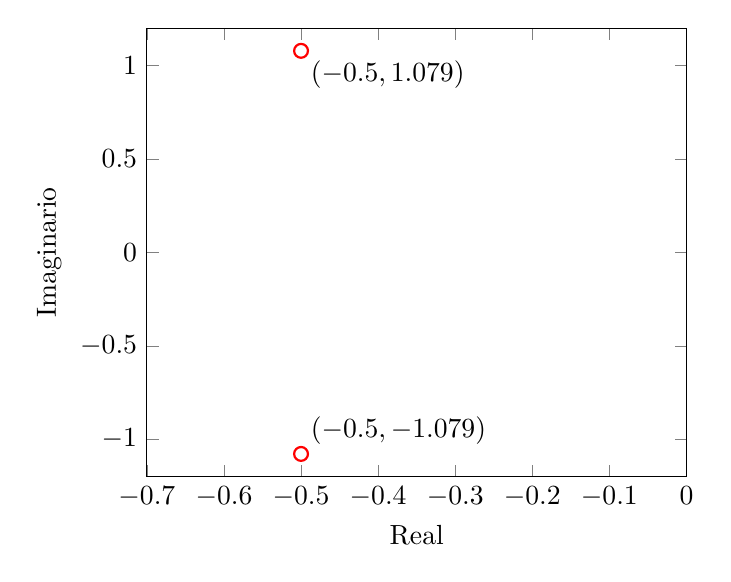
\begin{tikzpicture}
        \begin{axis}[
            xlabel = {Real},
            ylabel = {Imaginario},
            xmin = -0.7, xmax = 0,
            ymin = -1.2, ymax = 1.2
        ]
            \addplot[only marks, mark = o, red, thick, mark size = 2.5pt] coordinates {(-0.5, 1.079) (-0.5, -1.079)};
            \node at (-0.5, -1.079)[above right]{$(-0.5, -1.079)$};
            \node at (-0.5, 1.079)[below right]{$(-0.5, 1.079)$};
        \end{axis}
    \end{tikzpicture}
    \caption{Polos de $F(s)$}
    \label{polos:fs}
\end{figure}



\begin{figure}[ht!]
    \begin{lstlisting}[caption={Cálculo de los polos de la función $F(s)$}, label={codigo_polos_fs}]
    s = tf('s'); %si primero defino Fs me va a tirar error ya que no le estoy pasando
    % en formato array, en cambio si defino a 's' como una función
    % transferencia entonces ahí si me dejará
    Fs = exp(-s) / (s^2 + s + sqrt(2)); 
    polosFs = pole(Fs);
    [y, t] = step(Fs, 10);
    plot(t, y);
    \end{lstlisting}
\end{figure}


\newpage

\section{Lecciones aprendidas y Conclusión}
En este trabajo se empleó el uso del cálculo simbólico para respuestas de sistemas ante entradas escalón, sin necesidad de modelarlo en Simulink, aprovechando la rapidez y fácil curva de aprendizaje de usar cálculo simbólico. Además, se hizo uso de la función \texttt{tf()} para crear funciones de transferencias para luego generar un plot de las respuestas ante distintas entradas. 

En conclusión, la combinación de estas herramientas permite optimizar el flujo de trabajo para sistemas dinámicos, permitiendo aobrdar de forma precisa el comportamiento transitorio y la ubicación de polos y ceros sin incurrir en una alta carga computacional o de modelado.





\newpage
\thispagestyle{empty}
\bibliography{biblioteca.bib}
\bibliographystyle{plain}


\end{document}